\subsection{Performance Evaluation}
\label{sub:evaluation-performance}


\paragraph{Setup.} We configure two testbeds for performance evaluation. %to evaluate the performance of \prototype.
\begin{itemize}[leftmargin=*]
\item {\bf LAN.} It includes three machines, each of which is equipped with an eight-core 2.9\,GHz Intel Core i7-10700 CPU, a 4\,TB 7200 RPM Seagate Exos SATA hard disk drive and 32\,GB RAM.  All machines are connected via a 10\,Gbps switch, and run Ubuntu 20.04.3.

\item {\bf Cloud.} It is deployed in {\em Alibaba Cloud} \cite{alibaba}. We rent several {\em ecs.g7t.3xlarge} virtual machines (VMs) in two regions to run the cloud, key server and multiple clients, respectively. The VMs in the same and across different regions are connected with 10\,Gbps and 100\,Mbps networks, respectively.
  Each VM is equipped with a 12-core 3.5\,GHz CPU virtualized by an Intel Xeon (Ice Lake) Platinum 8369B and 48\,GiB memory, and installed with  Alibaba Cloud Linux 3.2104. We additionally mount the cloud machine with {\em Alibaba General-Purpose NAS} as the storage backend. The NAS can achieve up to 15K\,IOPS for 4\,K random reads and writes.
  %with 150\,MBps bandwidth.
\end{itemize}
  % Besides the LAN testbed, we also configured a Cloud testbed to evaluate the multiple-client performance in under both synthetic and real-world workloads. We select which supports Intel SGX in two different regions.  All machines run. The highest network bandwidth between instances in the same region is 10Gbps, while the network bandwidth between instances in the two regions is 100 Mbps. And, we use

We make the following default configuration. For the underlying \sysnameF, we fix $W$ = 5\,K (i.e., about 300\,KiB EPC usage), $T$ = 3\%, the size of the similarity indicator at 32\,bytes (i.e., two blocks), and the number of features extracted via N-transform as three. For \prototype, we configure three threads to extract the content features of plaintext chunks (except Exp\#5 that microbenchmarks the performance of \prototype in a single thread, and Exp\#6 that evaluates the performance of \prototype using a varying number of threads to extract content features), and a 1\,GiB container cache to improve the download performance (\S\ref{sec:implementation}).

\subsubsection{Synthetic Workloads}
\label{subsub:syn}

We evaluate \prototype using SYNUnique, in which each 2\,GiB file includes globally unique chunks (\S\ref{sub:datasets}).
To avoid disk I/O, we load all data into each client's memory before each test, and let the cloud store all received data in memory (as opposed to Exp\#8 that enables disk I/O to study real-cloud deployment).
Our goal is to understand the maximum achievable performance of \prototype without the impact of deduplication and disk I/O, and show that \prototype incurs limited performance overhead over SGXDedup \cite{ren21}.
We average the results of each experiment over 10 runs, and include the 95\% confidence intervals from {\em Student's t-Distribution} into bar charts (for brevity, we exclude them from line charts).

\paragraph{Exp\#5 (Microbenchmarks).}
We start with microbenchmark evaluation by deploying a client, a key server, and a cloud in distinct machines in the LAN testbed. We let the client upload the same 2\,GiB file in SYNUnique twice, and evaluate the processing time of different upload steps in a single thread. The considered steps include: (i) {\em chunking}, which partitions the input file into variable-size plaintext chunks; (ii) {\em feature generation}, which extracts the content features of each plaintext chunk and samples the target feature(s) based on \sysnameF instances; (iii) {\em fingerprinting}, which computes the fingerprint of each plaintext chunk; (iv) {\em key generation}, which generates both feature key and MLE key; (v) {\em encryption}, which encrypts each plaintext chunk; (vi) {\em detection}, which detects the learning-content attack based on ciphertext chunks; (vii) {PoW}, which proves the ownership of each ciphertext chunk; (viii) {\em deduplication}, in which the cloud detects duplicate chunks; (ix) {\em transfer}, which transmits non-duplicate ciphertext chunks and the file recipe.

% We present the time breakdown of \sysnameF to study the performance of different steps. (i) {\em chunking}, which divides the input file into non-overlapping plaintext chunks; (ii) {\em feature extraction} extracts the corresponding minFeature/firstFeature/allFeature from each chunk for feature-based key generation; (iii) {\em fingerprinting}, calculates the fingerprint of each chunk for MLE key generation; (iv) {\em key generation}, uses the key server to generate MLE key and feature-based key based on MLE hash and features; (v) {\em encryption}, use feature-based key to encrypt the indicator, and MLE key to encrypt the remaining content of each chunk; (vi) {\em detection}, the enclave launch attack detection based on the indicators; (vii) {\em SGX-based PoW}, which prove the ownership of the ciphertext chunk to the cloud; (viii) {\em deduplication}, in which the cloud detect duplicate chunks and inform the client; (ix) {\em transfer}, which uploads the non-duplicate ciphertext chunks and the recipe.

\begin{table}[t]
    \small
    \centering
    \setlength{\tabcolsep}{5pt}
    \renewcommand{\arraystretch}{1.05}
    \setlength{\tabcolsep}{0.006\textwidth}{
    \begin{tabular}{|c|c|c|c|c|}
        \hline
        \multicolumn{2}{|@{\,}c|}{\textbf{Procedure/Step}} & \multicolumn{1}{l|}{\hspace{.5em}\textbf{firstFeature}} &
        \multicolumn{1}{c|}{\textbf{minFeature}} &
        \multicolumn{1}{c|}{\textbf{allFeature}} \\ \hline \hline
        \multicolumn{2}{|c|}{Chunking} & \multicolumn{3}{c|}{$2.12\pm0.006$} \\ \hline
        \multicolumn{2}{|c|}{\makecell[c]{Feature generation}} &
        \makecell[c]{$4.34 \pm 0.01$} & \makecell[c]{$9.93 \pm0.04$} & \makecell[c]{$9.85 \pm0.02$} \\ \hline
        \multicolumn{2}{|c|}{\makecell[c]{Fingerprinting}}&
        \multicolumn{3}{c|}{$1.81 \pm 0.002$} \\ \hline        \multicolumn{2}{|c|}{\makecell[c]{Key generation}}&
        \multicolumn{3}{c|}{$0.73 \pm 0.02$ ($0.49 \pm 0.01$)} \\ \hline
        \multicolumn{2}{|c|}{Encryption} & \multicolumn{3}{c|}{$1.22 \pm 0.001$} \\ \hline
        \multirow{2}{*}{In Enclave}
        & Detection &
        \multicolumn{3}{c|}{$0.04   \pm 0.005$} \\ \cline{2-5}
        & PoW &
        \multicolumn{3}{c|}{$1.86   \pm 0.004$} \\ \hline
        \multicolumn{2}{|c|}{Deduplication}  &
        \multicolumn{3}{c|}{$0.55 \pm 0.02$}  \\ \hline
        \multicolumn{2}{|c|}{Transfer}  & \multicolumn{3}{c|}{$1.16 \pm 0.03$ ($0.04 \pm 0.001$)}\\ \hline
    \end{tabular}
    }
    \caption{(Exp\#5) Time breakdown per 1\,MiB of synthetic file data processed (unit: ms). Except explicitly specified in parentheses, the consumed time of each step in the second upload is identical with that in the first upload.}
    \label{tab:evaluation-syn-system-breakdown}
    \vspace{-6pt}
\end{table}

Table~\ref{tab:evaluation-syn-system-breakdown} presents the results (per 1\,MiB file data processed). Since \prototype builds on SGXDedup \cite{ren21}, it inherits the performance benefits to offload the computational overhead of key generation (\S\ref{sec:implementation}) in the second upload, as well as avoid the transfer of duplicate chunks. The detection step is efficient, and takes up to 0.4\% of the overall time in the upload procedure. In addition, the feature generation step is expensive due to the computational overhead of N-transform. For example, {\tt firstFeature} takes 31.4\% of the overall time in the first upload; the consumed time fractions further increase to  51.1\% and 50.9\% for
{\tt minFeature} and {\tt allFeature}, respectively, since they extract all three features (as opposed to {\tt firstFeature} that only extracts the first feature). However, we argue that we can mitigate the performance overhead of feature generation via multi-threading (see below).




% Here we perform two consecutive uploads of the same synthetic file (2GiB random file) to verify the difference in system performance when uploading non-duplicate and duplicate data. Since \sysnameF is developed based on {\em SGXDedup}, we have retained all the features in SGXDedup. Therefore, in the second upload, the key generation step's time computation decreased by $49\%$ (this is due to the speculative encryption in SGXDedup could off-line generate encryption/decryption mask for future key generation requests). At the same time, since the second upload does not require any ciphertext chunks to be uploaded, the time cost of uploading only the relevant metadata is only $3.45\%$ of the first upload.

% The detection step is very efficient, which only brings the overhead of $2\%$ to the enclave. However, feature extraction requires a lot of time (up to $51.13\%$ and $50.93\%$ of total time consumption with minFeature and allFeature, $31.38\%$ with firstFeature in the first upload), which will become the performance bottleneck of \sysnameF. Since the minFeature and allFeature schemes need to calculate a total of 3 features and then extract the target feature, but the firstFeature scheme only needs to calculate one feature, so it only needs $43.7\%$ of time to be completed. In the \sysnameF system, we use multiple threads to perform feature extraction calculations in parallel to reduce the overall system overhead.

\paragraph{Exp\#6 (Single-client performance).}
We consider a single client, and compare the performance of \prototype with the base system SGXDedup. We let the client upload the same file twice (like Exp\#5) and further download the file.
%We evaluate the upload (download) speed as the ratio of the file size (i.e., 2\,GiB) to the time the client finishes the upload (download).

Figure~\ref{fig:singleClientThroughput}(a) and Figure~\ref{fig:singleClientThroughput}(b) present the upload speeds of the first and second uploads, respectively, when we vary the number of threads to extract features (\S\ref{sec:implementation}). The speed of SGXDedup keeps as 297.1\,MiB/s in the first upload, and 304.3\,MiB/s in the second upload, since it does not extract features. The upload speed of \prototype first increases with the number of threads (e.g., 265.3\,MiB/s for {\tt firstFeature}, 261.3\,MiB/s for {\tt minFeature} and 262.6\,MiB/s for {\tt allFeature} when three threads are used to extract features in the first upload), and then decreases (e.g., at about 220\,MiB/s in the first upload and 225\,MiB/s in the second upload for all three instances) due to resource contention. By exploiting multi-threading, \prototype only incurs the performance overhead over SGXDedup at 8.0-12.0\% in the first upload, and 6.6-7.5\% in the second upload.
In addition, we  observe few performance differences between the first and second (that does not need to transfer duplicate data) uploads, since our LAN testbed has high  bandwidth for transferring data. We argue that source-based deduplication brings significant performance gains in real-cloud deployment (Exp\#8), and reduces the network traffic for processing real storage workloads (Exp\#10).
Figure~\ref{fig:singleClientThroughput}(c) compares the download speed. \prototype incurs 1.3\% performance drop, since it decrypts each chunk with both the MLE key and the feature key.


% We consider a single client, and compare the upload and download performance of \prototype with the baseline system: SGXDedup, which adopts SGX-based server-aided MLE generation and SGX-based PoW to support source-based deduplication with high security and performance. Note that, we build \prototype based on the baseline SGXDedup system. Therefore, we retained all the features of SGXDedup, especially speculative encryption which could boost the key generation performance when the system is not used for the first time. We evaluate the upload and download speeds in three cases: (i) a client first uploads a 2\, GiB file;  (ii) the client restarts and then uploads the identical 2\, GiB file again; and (iii) the client downloads the file. We first analyze the effect of multi-threaded feature extraction optimization through the first round of upload, then analyze the optimization effect of SGXDedup's design on duplicate data upload through the second round of upload, and finally analyze the impact of encrypting indicators separately on download performance. To analysis the theoretical performance of \prototype, we conduct the performance test in the ramdisk and run the test 10 times to give the confidence interval in student-t distribution.

\begin{figure}[t]
    \centering
    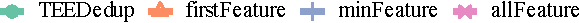
\includegraphics[width=0.35\textwidth]{pic/featurespy/plot/performance/LANSyn/legend.pdf}\\
    \vspace{1pt}
    \begin{tabular}{@{\ }c@{\ }c@{\ }c}
        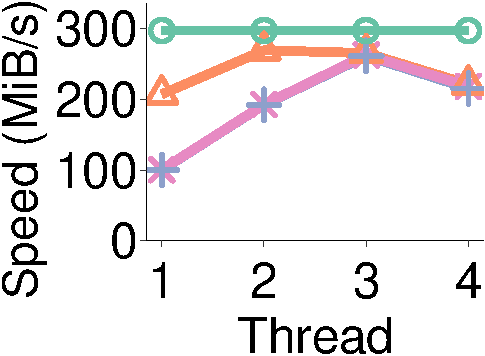
\includegraphics[height=.78in]{pic/featurespy/plot/performance/LANSyn/upload_thread_line.pdf}&
        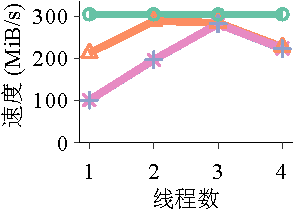
\includegraphics[height=.78in]{pic/featurespy/plot/performance/LANSyn/upload_thread_2nd_line.pdf}&
        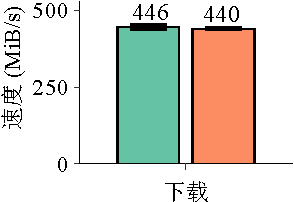
\includegraphics[height=.78in]{pic/featurespy/plot/performance/LANSyn/download_bar.pdf}\\
        \makecell[c]{\small (a) 1st upload} &
        \makecell[c]{\small (b) 2nd upload} &
        \makecell[c]{\small (c) Download}\\
    \end{tabular}
    \vspace{-6pt}
    \caption{(Exp\#6) Single-client performance in the LAN testbed. In download, all \prototype instances achieve the same speed, and we compare them (orange) with SGXDedup (green).}
    \vspace{-6pt}
    \label{fig:singleClientThroughput}
\end{figure}


\paragraph{Exp\#7 (Multi-client performance).}
We evaluate the performance when multiple clients issue uploads/downloads concurrently. We use the cloud testbed to consider an increasing number of clients, and deploy all clients, the key server and the cloud in the same region. We measure the {\em aggregate upload (download) speed} as the ratio of the total uploaded (downloaded) data size to the total time all clients finish the uploads (downloads).


\begin{figure*}[t]
    % \hspace{-5pt}
    \begin{minipage}[t]{0.58\textwidth}
        \centering
        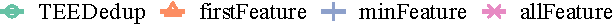
\includegraphics[width=0.7\linewidth]{pic/featurespy/plot/performance/multiClient/legend.pdf}\\
        \vspace{1pt}
        \begin{tabular}{@{\ }c@{\ }c@{\ }c}
            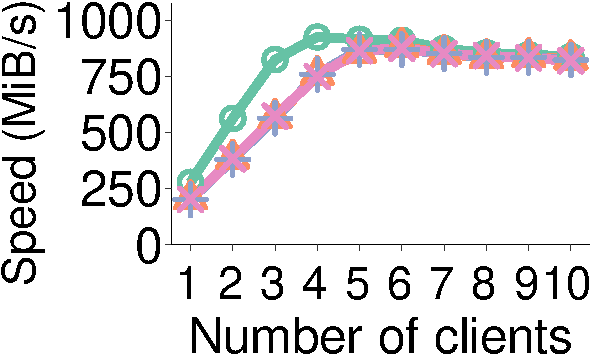
\includegraphics[width=0.32\linewidth]{pic/featurespy/plot/performance/multiClient/upload_1st_line.pdf}&
            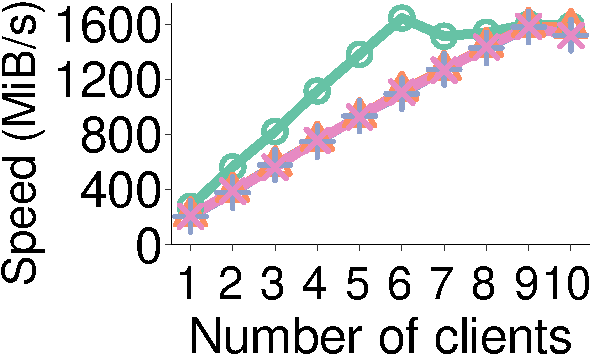
\includegraphics[width=0.32\linewidth]{pic/featurespy/plot/performance/multiClient/upload_2nd_line.pdf}&
            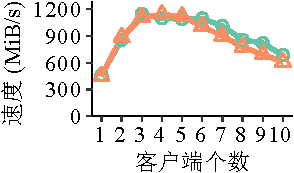
\includegraphics[width=0.32\linewidth]{pic/featurespy/plot/performance/multiClient/download_line.pdf}\\
            \makecell[c]{\small (a) 1st upload} &
            \makecell[c]{\small (b) 2nd upload} &
            \makecell[c]{\small (c) Download}\\
        \end{tabular}
        \vspace{-11pt}
        \captionof{figure}{(Exp\#8) Multi-client performance. The download speeds of all \prototype instances are identical, and we compare it (orange) with SGXDedup (green).}
        \vspace{-5pt}
        \label{fig:expMultiClientThroughput}
      \end{minipage}
          \hspace{6pt}
          \begin{minipage}[t]{0.4\textwidth}
               \vspace{-6pt}
               \centering

               \setlength{\tabcolsep}{0.01\textwidth}{
                 \small
          \begin{tabular}{|c|c|c|c|}
                \hline
                {\bf Approach} & {\bf 1st Upload} & {\bf 2nd Upload} & {\bf Download} \\
                \hline
                \hline
                Transfer & \multicolumn{3}{c|}{11.8 $\pm$ 0.04} \\
                \hline
                \hline
                \makecell[c]{\tt firstFeature} & \multirow{3}{*}{11.5 $\pm$ 0.006} & 204.4 $\pm$ 10.06 & \multirow{3}{*}{11.5 $\pm$ 0.004} \\
                \cline{1-1}\cline{3-3}
                \makecell[c]{\tt minFeature} &  & 184.7$\pm$ 7.4 &  \\
                \cline{1-1}\cline{3-3}
                \makecell[c]{\tt allFeature} &  & 185.0$\pm$ 6.4 &  \\
                \hline
                SGXDedup & 11.5 $\pm$ 0.009 & 233.2 $\pm$ 8.4 & 11.5 $\pm$ 0.004 \\
                \hline
            \end{tabular}
        }
        \hspace{15pt}
        \vspace{2pt}
        \captionof{table}{(Exp\#7) Real-cloud deployment (unit: MiB/s). We use {\tt scp} to upload a 2\,GiB file from the client to the cloud to provide a transfer benchmark in the environment.}
        \label{tab:expCloudTest}
      \end{minipage}
\end{figure*}

Figure~\ref{fig:expMultiClientThroughput} presents the results with up to 10 clients. We do not consider more clients, since the aggregate upload speed has  generally become stable. Specifically, the speeds of both the first and the second uploads  increase with the number of clients, and then gradually decrease due to the write contention at the cloud. We observe that SGXDedup reaches the peak performance (e.g., at 924.9\,MiB/s for four clients in the first upload) earlier than \prototype (e.g., up to 882.2\,MiB/s for six clients in the first upload), since it achieves high performance and the cloud is easy to be saturated. Similarly, the download speeds of all approaches decrease beyond three (for SGXDedup that achieves the peak speed of 1148.7\,MiB/s) or four (for \prototype that achieves the peak speed of 1141.3\,MiB/s) clients due to the read contention in the cloud.



% for at most 12 clients. Here, we present: (a) the aggregated first-round upload speed of the \prototype's three schemes and SGXDedup; (b) the second round aggregated upload speed of uploading duplicate data; (c) the aggregated download speed of SGXDedup and \prototype. We found that similar to Exp\#7, in the case of only one client, in the first round of upload, firstFeature, minFeature, and allFeature based \prototype brought $26.9\%$, $27.9\%$ and $27.3\%$ overheads to SGXDedup, respectively. While in the second round, they brought $25.1\%$, $25.6\%$, and $25.7\%$ overhead compared with SGXDedup, which is slightly lower than the overhead in the first round upload. For firstFeature-based scheme, the key generation is the bottleneck of \prototype, while SGXDedup only needs half of the key generation cost which will not become a bottleneck (See Exp\#11 for detailed Intranet deployment breakdown). Note that we set the key enclave to optimize second-round key generation for 12 clients. So, only about $\sim20\%$ of the data of each client can be accelerated by the SGX-based speculative encryption, which can only slightly reduce the overhead, but key generation is still the bottleneck of firstFeature-based \prototype. At the same time, minFefature and allFeature based \prototype's performance is severely restricted by feature generation.


% We consider multiple clients for upload and download operations. Same as Exp\#6, we test its peak performance in ramdisk. To collect the results of more clients, we deployed the key server and the cloud and all clients in the same region in the Alibaba Cloud and used the intranet for testing, which bandwidth is 10Gbps. We start all clients at the same time and count the time required for the last completed client to calculate the total system throughput of multiple clients.

% \begin{figure*}[t]
%     \centering
%     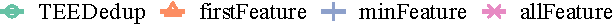
\includegraphics[width=0.4\textwidth]{pic/featurespy/plot/performance/multiClient/legend.pdf}\\
%     \vspace{1pt}
%     \begin{tabular}{@{\ }c@{\ }c@{\ }c}
%         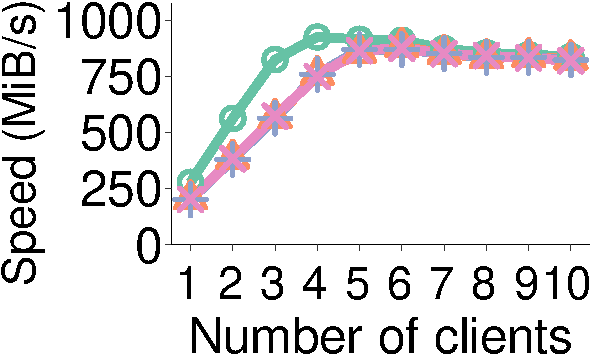
\includegraphics[width=0.33\textwidth]{pic/featurespy/plot/performance/multiClient/upload_1st_line.pdf}&
%         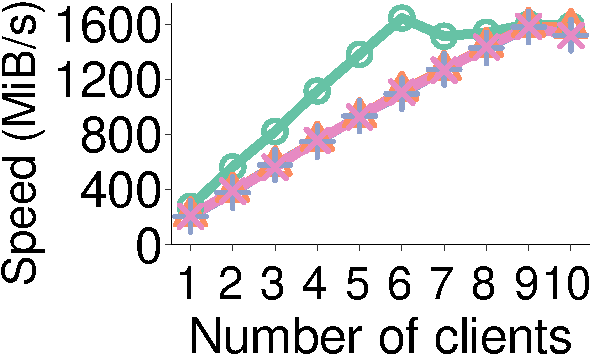
\includegraphics[width=0.33\textwidth]{pic/featurespy/plot/performance/multiClient/upload_2nd_line.pdf}&
%         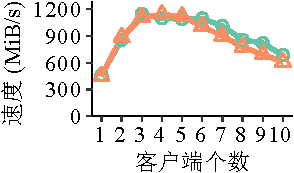
\includegraphics[width=0.33\textwidth]{pic/featurespy/plot/performance/multiClient/download_line.pdf}\\
%         \makecell[c]{(a) 1st round upload} &
%         \makecell[c]{(b) 2nd round upload} &
%         \makecell[c]{(c) Download}\\
%     \end{tabular}
%     \vspace{-5pt}
%     \caption{(Exp\#8) Multi-client uploads and downloads. (a)Compares the aggregated first-round upload speed of the \prototype's three schemes and SGXDedup with different number of clients. (b) Compares the aggregated speed of uploading duplicate data in the second round with different number of clients. (c) Compares the aggregated download speed of SGXDedup and \prototype}
%     \vspace{-5pt}
%     \label{fig:expMultiClientThroughput}
% \end{figure*}


% With the increase in the number of clients, the aggregated throughput of the two rounds of uploads both rose rapidly and then slightly declined. In the first round of upload, the peak of SGXDedup appeared at 4 clients ($924.9$\,MiB/s), and the peak of \prototype appeared when there are 6 clients (average $875.6$\,MiB/s for three schemes), this is because the client performance of \prototype is lower than SGXDedup, and the server write contention aggravate late. In the second round, the peak of SGXDedup appeared when there were 6 clients ($1644.4$\,MiB/s), and \prototype's maximum speed appeared with 9 clients (average $1581.7$\,MiB/s for three schemes). The number of clients at peak performance has increased. It is because the second round does not need to upload duplicate data, which reduced the cloud's write contention, and the system throughput is only limited by deduplication query. For downloading, the \prototype reached peak performance ($1141.3$\,MiB/s) with 4 clients, and SGXDedup reached peak performance ($1148.7$\,MiB/s) with 3 clients. And the download throughput of SGXDedup under each client number is slightly higher than \prototype, this is because the client pressure of \prototype is slightly higher than that of SGXDedup during downloading. After reaching the peak performance, both SGXDedup and \prototype is affected by cloud read contention and decline quickly.




\paragraph{Exp\#8 (Real-cloud deployment).}
We extend Exp\#6 to study the single-client performance in the cloud testbed. We deploy the client and the key server in two VMs in the same region, and a cloud in a different region (as opposed to Exp\#7, in which all entities are deployed in the same region), so as to simulate the scenario that Internet is connected between  the client and the cloud. Also, we let the client read the file from the local disk (i.e., SSD that achieves about 270\,MiB/s for reads/writes) for uploads, and the cloud store received data in the attached NAS. We use {\tt scp} to benchmark the transfer speed between the client and the cloud.



%read the file from the disk and upload it (for comparison, Exp\#6 load the file into the ramdisk and then upload it), and let the cloud store the received data in the NAS. We also use {\em scp} to upload the same 2\,GiB file as the benchmark of the Internet environment.

% based on Exp\#6, we deploy \prototype and SGXDedup in a real cloud environment. To avoid the impact of fluctuations in the local network environment, we deploy cloud at region A and deploy client and key server at region B to simulate real data outsourcing scenarios. The network bandwidth between the two Cloud (\S\ref{sub:evaluation-performance}) region is 100 Mbps.

% \begin{table}[t]
%     \small
%     \centering
%     \renewcommand{\arraystretch}{1.05}
%     \begin{tabular}{|c|c|c|c|}
%     \hline
%     {\bf Approach} & {\bf First Upload} & {\bf Second Upload} & {\bf Download} \\
%     \hline
%     \hline
%     Transfer & \multicolumn{2}{c|}{11.84 $\pm$ 0.04} & \multicolumn{1}{c|}{11.56 $\pm$ 0.19}  \\
%     \hline
%     \hline
%     \makecell[c]{firstFeature} & \multirow{3}{*}{11.46 $\pm$ 0.006} & 204.44 $\pm$ 10.057 & \multirow{3}{*}{11.45 $\pm$ 0.004} \\
%     \cline{1-1}\cline{3-3}
%     \makecell[c]{minFeature} &  & 184.71$\pm$ 7.415 &  \\
%     \cline{1-1}\cline{3-3}
%     \makecell[c]{allFeature} &  & 184.96$\pm$ 6.387 &  \\
%     \hline
%     SGXDedup & 11.51 $\pm$ 0.009 & 233.22 $\pm$ 8.358 & 11.54 $\pm$ 0.004 \\
%     \hline
%     \end{tabular}
%     % \vspace{-1pt}
%     \caption{(Exp\#7) Real-cloud upload and download (unit: MiB/s).}
%     \label{tab:expCloudTest}
%     \vspace{-6pt}
% \end{table}

Table~\ref{tab:expCloudTest} shows the results. In the first upload, the performance of all approaches is bounded by the transfer speed. In the second upload, the performance of SGXDedup and {\tt firstFeature} is bounded by chunking (Table~\ref{tab:evaluation-syn-system-breakdown}), while {\tt firstFeature} incurs 12.3\% performance overhead over SGXDedup, since it additionally extracts the first feature for key generation. The performance of both {\tt minFeature} and {\tt allFeature} (in the second upload) is bounded by features extraction. Note that the second upload speeds of all approaches are slower than those (Exp\#6) in the LAN testbed for three reasons. First, we now process on-disk files and enable disk I/O. Also, the VMs in the cloud testbed are virtualized from physical machines, and may incur performance drops when handling computational intensive operations.
Furthermore, the high latency of Internet slows down the  transferring of fingerprints in deduplication.
In the download, the performance of all approaches is bounded by the transfer speed, and \prototype incurs 0.6\% overhead when compared with SGXDedup.


% In the first round of upload, limited by the Internet bandwidth, the speeds of \prototype and SGXDedup are $11.46\pm 0.006$, and $11.51\pm 0.009$\,MiB/s, respectively. In the second round of uploading, \prototype (firstFeature) reached 204.44 $\pm$ 10.057\,MiB/s, while minFeature and allFeature are slightly slower than firstFeature scheme with 184.71$\pm$ 7.415\,MiB/s and 184.96$\pm$ 6.387\,MiB/s, respectively. For comparison, SGXDedup reached 233.22 $\pm$ 8.358\,MiB/s. Here, the overhead of \prototype firstFeature scheme compared with SGXDedup has reached $12.34\%$, which is higher than $6.48\%$ in Exp\#6. This is because the deduplication query (bound with the detection and SGX-based PoW) becomes the bottleneck of both SGXDedup and firstFeature-based \prototype, but firstFeature-based \prototype has additional data exchange overhead with multi-threaded feature generation. Meanwhile, the performance of minFeature and allFeature schemes is limited by feature generation (Refer to the breakdown for Internet deployment in Exp\#11), and the overhead compared with SGXDedup has reached $20.8\%$ and $20.7\%$ respectively. In download, \prototype and SGXDedup are restricted again by the Internet bandwidth, and the speeds are $11.47\pm 0.01$\,MiB/s and $11.54\pm 0.01$\,MiB/s respectively. Note that \prototype's download performance is slightly lower than SGXDedup by $0.6\%$, this is because the recipe in \prototype contains the feature-based key, which requires more processing time before download chunks.'



\subsubsection{Real-world Workloads}
\label{subsub:real}
We evaluate \prototype using FSL and MS, in order to understand its performance when processing real-world large-scale data.

\paragraph{Exp\#9 (Trace-driven performance).}
We evaluate the upload and download performance in the LAN testbed. We choose ten snapshots from FSL and MS each as follows. For FSL, we pick the weekly snapshots from the same user to have high cross-snapshot redundancies; For MS, we pick the snapshots that have the most intra-snapshot redundancies. The chosen FSL and MS snapshots take 407.5\,GiB and 902.5\,GiB of pre-deduplicated data, respectively. Since our snapshots only contain chunk fingerprints and sizes (\S\ref{sub:datasets}), we reconstruct each plaintext chunk by repeatedly writing its fingerprint into a spare chunk with the corresponding specified size. We first upload the snapshots one by one, and then download them in the same order of upload. Note that the original SGXDedup \cite{ren21} does not have the container cache (\S\ref{sec:implementation}); for fair comparison, we implement an in-memory cache for SGXDedup to buffer the most recently restored containers, and configure it with the same size (1\,GiB) as that of \prototype.


\begin{figure}[t]
    \centering
    
\includegraphics[height=0.15in]{pic/featurespy/plot/performance/LANTrace/trace_legend_upload.pdf}\\
    
\includegraphics[height=0.15in]{pic/featurespy/plot/performance/LANTrace/trace_legend_download.pdf}\\
    \vspace{3pt}
    \begin{tabular}{@{\ }c@{\ }c}
        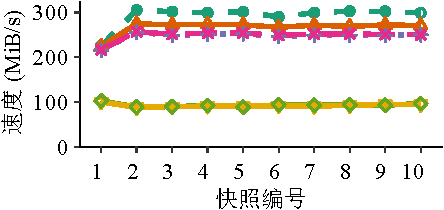
\includegraphics[height=.82in]{pic/featurespy/plot/performance/LANTrace/trace_fsl.pdf}&
        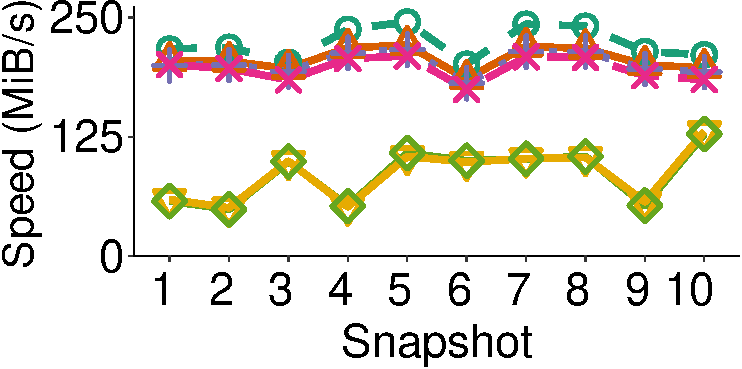
\includegraphics[height=.82in]{pic/featurespy/plot/performance/LANTrace/trace_ms.pdf}\\
        \mbox{\small (a) FSL} &
        \mbox{\small (b) MS}\\
        % 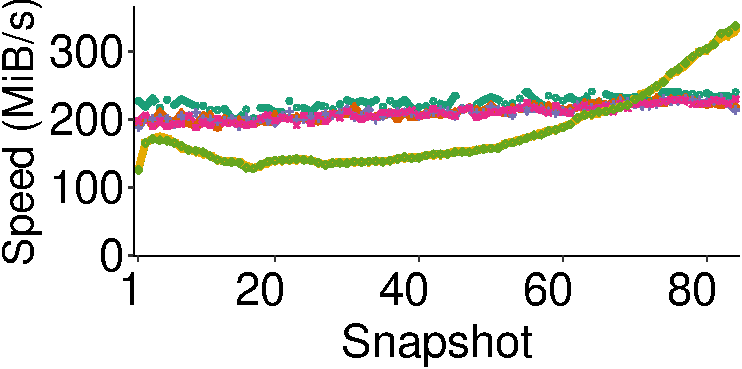
\includegraphics[height=.82in]{pic/featurespy/plot/performance/LANTrace/trace_linux.pdf}&
        % 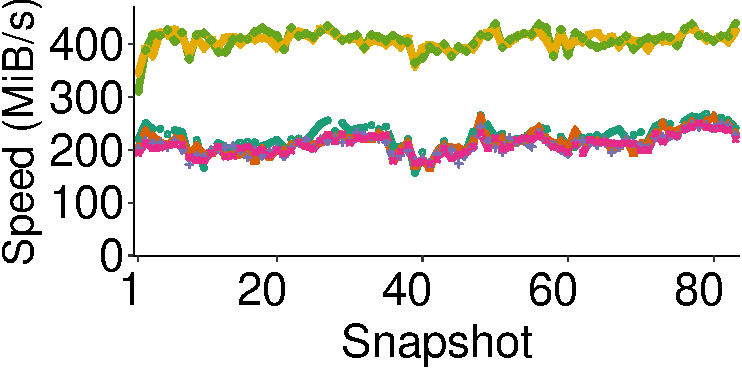
\includegraphics[height=.82in]{pic/featurespy/plot/performance/LANTrace/trace_couch.pdf}\\
        % \mbox{\small (c) Linux} &
        % \mbox{\small (d) CouchDB}\\
    \end{tabular}
    \vspace{-6pt}
    \caption{(Exp\#9) Trace-driven performance.}
    \vspace{-6pt}
    \label{fig:traceDrivenThroughput}
\end{figure}

Figure~\ref{fig:traceDrivenThroughput} presents the results. After the first FSL snapshot (e.g., 224.8\,MiB/s, 223.9\,MiB/s, 214.9\,MiB/s and 216.9\,MiB/s for SGXDedup, {\tt firstFeature}, {\tt minFeature} and {\tt allFeature}, respectively), both SGXDedup and \prototype achieve high performance (e.g., at least 298.9\,MiB/s, 266.8\,MiB/s, 246.4\,MiB/s  and 248.8\,MiB/s for SGXDedup, {\tt firstFeature}, {\tt minFeature} and {\tt allFeature}, respectively), since they do not need to transfer the cross-snapshot redundancies that take a large fraction in FSL. The download speed is generally steady (e.g., 88.7-102.6\,MiB/s for SGXDedup,  and 88.0-100.2\,MiB/s for \prototype). On average, compared to SGXDedup, {\tt firstFeature}, {\tt minFeature} and {\tt allFeature} slow down the upload performance by 8.8\%, 15.7\% and 15.0\%, respectively, and the download performance by 0.8\%.

Compared to FSL, the upload  performance in MS generally drops by about 21\%, since MS includes many unique chunks and leads to a large fingerprint index (that is implemented via LevelDB \cite{leveldb}). This aggravates the overhead of querying the fingerprint index for the existence of ciphertext chunks for deduplication. Also, the download speed in MS fluctuates across snapshots, since some snapshots have more non-duplicate chunks and may be stored in the consecutive regions (i.e., less fragmented \cite{lillibridge13}) that can be quickly accessed via sequential reads.



% (a) shows the upload and download speeds across FSL snapshots. Both SGXDedup and \prototype can achieve high upload speeds. When uploading the first snapshots, SGXDedup achieves $224.8$\, MiB/s upload speed, while \prototype achieves average speed at $218.6$\, MiB/s, and then when uploading the remaining snapshots, due to a large number of duplicate chunks, the upload speeds of SGXDedup and \prototype are significantly improved. For \prototype and SGXDedup, the average performance of $257.9$\, MiB/s and $300.1$\, MiB/s has bEen reached respectively. On average, \prototype incurs an upload performance drop of $13.18\%$ compared to SGXDedup. Note that the overhead is slightly larger than that ($5.26\%\sim7.23\%$) in our synthetic performance evaluation (Exp\#6). The reason is that chunking is now disabled in trace-driven evaluation, the bottleneck of SGXDedup has changed from chunking to SGX-based PoW, and the upper-performance limit has been improved, but the bottleneck of \prototype is still the feature extraction.  The download speed decreases from $102.6$\,MiB/s to $88.7$\,MiB/s for SGXDedup, and from $100.2$\,MiB/s to $88.0$\,MiB/s for \prototype, mainly due to the decrease in cache hit rate caused by chunk fragmentation \cite{lillibridge13}.

% Figure~\ref{fig:traceDrivenThroughput}(b) shows the upload and download speeds across MS snapshots. Both systems achieve lower upload speeds than in the FSL snapshots since the MS dataset has larger data volume and increased the access overhead of the fingerprint index. On average, \prototype incurs upload overhead of $9.65\%$ compared to SGXDedup. Note that the download speed of the MS dataset fluctuates greatly, because the deduplication ratio between each snapshot of MS is low and the difference is obvious, the hit rate of our container cache fluctuates greatly.

\paragraph{Exp\#10 (Network traffic analysis).}
We analyze the network traffic of \prototype, and compare it with three deduplication approaches that are secure against the learning-content attack: (i) {\em target-based deduplication} \cite{harnik10}, which forces the client to transfer all ciphertext chunks to the cloud; (ii) {\em random-threshold deduplication} \cite{harnik10}, which performs target-based deduplication if the number of uploads of each chunk is smaller than a pre-defined threshold, or source-based deduplication (\S\ref{sub:basics}) otherwise; (iii) {\em two-stage deduplication} \cite{li15}, which performs source-based deduplication on the ciphertext chunks from the same client, followed by target-based deduplication on those across different clients. Here, we follow the previous work \cite{harnik10} to choose the upper and lower bounds of the threshold in randomized-threshold deduplication at 20 and 2, respectively. We focus on FSL and MS. For FSL, we merge the snapshots of each user on a daily basis, and store them in the order of time. For MS, we consider that each snapshot is from an individual client, and store the snapshots in the order of the snapshot ID.
We do not consider the bandwidth overhead due to file recipes.


% Here we only consider the network traffic generated by the fingerprint (32\,Byte) required for source-based deduplication and the chunks that need to be uploaded.

% We analyze the network traffic of \prototype during upload. We consider three schemes that can prevent learning-content attacks for comparison. They are all based on source-based deduplication (i.e., the client performs deduplication and only upload non-duplicate chunks to the cloud) and/or target-based deduplication (i.e., the client uploads all chunks to the cloud, which performs deduplication on the received chunks) schemes: (i) {\em two-stage deduplication} \cite{li15}, which applies source-based deduplication on each client, followed by target-based deduplication across clients; (ii) {\em randomized-threshold deduplication} \cite{harnik10}, which performs either source-based deduplication or target-based deduplication based on a randomly chosen threshold. Here, we  For FSL, as  For MS, Linux and CouchDB, we . Note that, CouchDB contains three different distributions, we upload the common version first, then the community version, and finally the enterprise version. For {\em two-stage deduplication}, we consider each different ID (in MS dataset) or version number (in Linux and CouchDB datasets) as an independent user.

\begin{figure}[t]
    \centering
    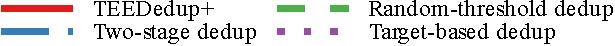
\includegraphics[height=0.2in]{pic/featurespy/plot/bandwidth/upload_traffic_legend.pdf}     \vspace{3pt} \\
    \begin{tabular}{@{\ }c@{\ }c}
        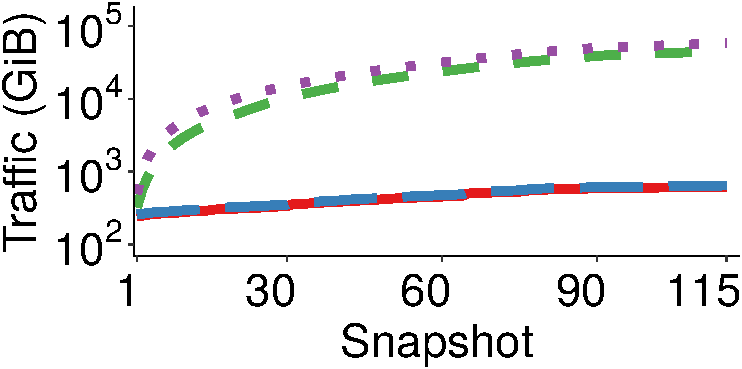
\includegraphics[width=0.23\textwidth]{pic/featurespy/plot/bandwidth/upload_traffic_fsl.pdf} &
        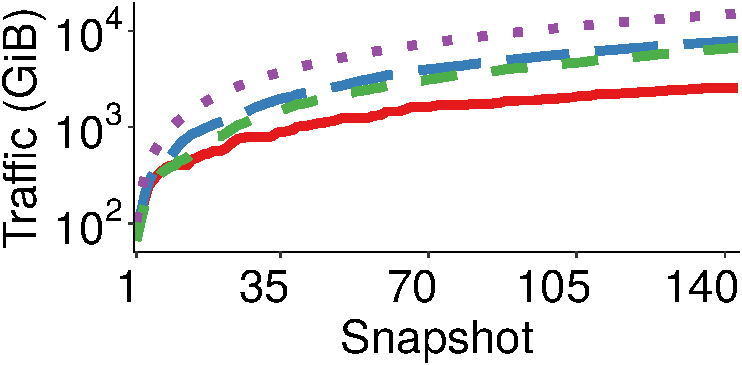
\includegraphics[width=0.23\textwidth]{pic/featurespy/plot/bandwidth/upload_traffic_ms.pdf} \\
        {\small (a) FSL} & {\small (b) MS} \\
        % 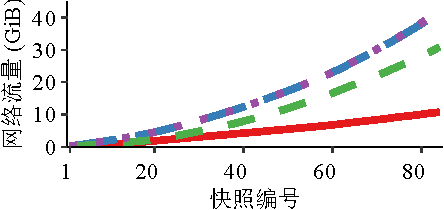
\includegraphics[width=0.23\textwidth]{pic/featurespy/plot/bandwidth/upload_traffic_linux.pdf} &
        % 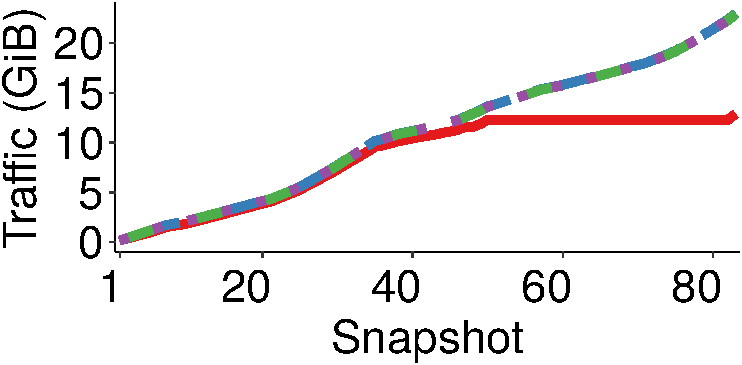
\includegraphics[width=0.23\textwidth]{pic/featurespy/plot/bandwidth/upload_traffic_couch.pdf} \\
        % {\small (c) Linux} & {\small (d) CouchDB}
    \end{tabular}
    \vspace{-6pt}
    \caption{(Exp\#10) Cumulative network traffic after storing each snapshot.}
    \vspace{-6pt}
    \label{fig:expNetworkTraffic}
\end{figure}


Figure~\ref{fig:expNetworkTraffic} presents the results. Since \prototype performs pure source-based deduplication, it outperforms the other approaches. For example, after storing the last snapshot, \prototype reduces the network traffic of target-based deduplication by 98.9\% in FSL and 83.1\% in MS. Two-stage deduplication performs well in FSL (e.g., only 3.7\% bandwidth overhead over \prototype), since FSL includes a large volume of intra-user redundancies. However, in MS, the network traffic of two-stage deduplication is finally 3.1$\times$ of that of \prototype. Random-threshold deduplication incurs varying network traffic in FSL (e.g., 72.5$\times$ of \prototype) and MS (e.g., 2.6$\times$ of \prototype).


% reduces the network traffic of target-based deduplication, random-threshold deduplication and two-stage deduplication
% Compared to
% shows the accumulated network traffic according to the snapshot storage order. When snapshots are uploaded, compared with target-based deduplication, \prototype saved $98.92\%$, $83.13\%$, $74.53\%$, and $43.78\%$ network traffic for FSL, MS, Linux, and CouchDB dataset respectively. Two-stage deduplication achieves almost the same traffic savings in FSL as $98.88\%$, because the FSL dataset includes a large volume of intra-user redundancies. In contrast, in the MS datasets, it can only achieve network traffic savings of $47.81\%$ (compare with \prototype, reduced by $42.48\%$). Since there is almost no redundancy in each version of the Linux and CouchDB datasets, and it requires a large number of source-based deduplication queries, for Linux, it only brings $1.05\%$ traffic savings, and for CouchDB, it even causes $0.31\%$ extra traffic overhead. The traffic savings brought by the Randomized-threshold deduplication are quite different. In MS, it brought $55.75\%$ traffic savings, while in FSL and Linux, there is only $21.60\%$ and $26.68\%$. However, it even introduces the extra traffic overhead of $0.0016\%$ in CouchDB. In addition, we found that in the first 35 versions of CouchDB, the network traffic of several schemes is almost the same, and for the latter versions, \prototype's accumulative network traffic keeps almost level. This is because these 35 versions are common versions with almost no redundancy. And there is a lot of redundancy between these common versions and the community/enterprise versions, making \prototype no longer need to upload a lot of data.
